\documentclass[12pt,letterpaper]{article}
\usepackage{fullpage}
\usepackage[top=2cm, bottom=4.5cm, left=2.5cm, right=2.5cm]{geometry}
\usepackage{amsmath,amsthm,amsfonts,amssymb,amscd}
\usepackage{lastpage}
\usepackage{enumerate}
\usepackage{fancyhdr}
\usepackage{mathrsfs}
\usepackage{xcolor}
\usepackage{graphicx}
\usepackage{listings}
\usepackage{hyperref}
\usepackage{graphicx}
\usepackage{tikz}

\hypersetup{%
  colorlinks=true,
  linkcolor=blue,
  linkbordercolor={0 0 1}
}
 
\renewcommand\lstlistingname{Algorithm}
\renewcommand\lstlistlistingname{Algorithms}
\def\lstlistingautorefname{Alg.}

\lstdefinestyle{Python}{
    language        = Python,
    frame           = lines, 
    basicstyle      = \footnotesize,
    keywordstyle    = \color{blue},
    stringstyle     = \color{green},
    commentstyle    = \color{red}\ttfamily
}

\setlength{\parindent}{0.0in}
\setlength{\parskip}{0.05in}

% Edit these as appropriate
\newcommand\course{CSE 3500}
\newcommand\hwnumber{2}                  % <-- homework number
\newcommand\NetIDa{bec19009}           % <-- NetID of person #1

\pagestyle{fancyplain}
\headheight 35pt
\lhead{\NetIDa}
\chead{\textbf{\Large Homework \hwnumber}}
\rhead{\course \\ \today}
\lfoot{}
\cfoot{}
\rfoot{\small\thepage}
\headsep 1.5em

\begin{document}

\begin{center}
    \LARGE Divide-and-conquer problem set
\end{center}

\section*{Problem 0}

Give upper $(O(\cdot))$ asymptotic bounds for the following recurrences. You may assume a $O(1)$
base case for small $n$. Justify your answer by some combination of the following: deriving
how much total work is done at an arbitrary level $k$, how many levels there are, and how
much work is required to merge (function body). For each recurrence, state whether or not
it is top-heavy, bottom-heavy, or even work. Answers that only cite the Master theorem will
not receive full credit.

\begin{enumerate}
    \item{$T(n) = 2T(\frac{n}{2})+O(n)$}
    \item{$T(n) = 2T(\frac{n}{2})+O(1)$}
    \item{$T(n) = 7T(\frac{n}{2})+O(n^3)$}
    \item{$T(n) = 7T(\frac{n}{2})+O(n^2)$}
    \item{$T(n) = 4T(\frac{n}{2})+O(n^2\sqrt{n})$}
    \item{$T(n) = 4T(\frac{n}{2})+O(n\log_2(n))$}
\end{enumerate}

For each of the following problems, we can infer a base case when $n = 1$ then the output would be $1$.
This is because for any of these problems, if there is only one element then only that element needs to be cheked.

\begin{enumerate}
    \item We can create a equation for each level $k$ of the recusion tree by finding what each levels equation is. Our first level down 
    can be derived from what $T(\frac{n}{2})$ is equal to.
    We can do this by dividing $2T(\frac{n}{2})+n$ by 2 which gets us $2T(\frac{n}{2^2})+\frac{n}{2}$. We can then
    then plug this into the original equation of $2T(\frac{n}{2})+n$ to get $2[2T(\frac{n}{2^2}) + \frac{n}{2}] + n$ which
    simplifies to $2^2T(\frac{n}{2^2}) + 2n$. We can use this process to find what $T(\frac{n}{2^3})$ is and from that, plug that
    into the equation to get $2^3T(\frac{n}{2^3}) + 3n$. We can repeat this process until we get to $T(n) = 2^kT(\frac{n}{2^k}) + kn$
    where $k$ is the number of levels in the recursion tree. We can now also assume $T(\frac{n}{2^k})$ is trying to reach $1$ which is the base case.
    We now solve for $k$ from $T(\frac{n}{2^k}) = T(1)$ to get 
    $n = 2^k$ which gives us $k = \log_2(n)$. We can now plug this into the equation to get $T(n) = 2^{\log_2(n)}T(1) + n\log_2(n)$ which
    simplifies down to $T(n) = nT(1) + n\log(n)$ or $T(n) = O(nlog(n))$. This is a top-heavy recusion because the work done at each
    level is $O(n)$ and the number of levels is $O(\log(n))$. This means that the total work done is $O(n\log(n))$.
    \item Just like the previous questions, we can create a equation for each level $k$ of the recusion tree by finding what $T(\frac{n}{2})$ is equal to.
    We can do this by dividing $2T(\frac{n}{2})+1$ by 2 which gets us $2T(\frac{n}{2^2})+\frac{1}{2}$. We can then
    then plug this into the original equation of $2T(\frac{n}{2})+1$ to get $2[2T(\frac{n}{2^2}) + \frac{1}{2}] + 1$ which
    simplifies to $2^2T(\frac{n}{2^2}) + 2$. We can repeat this process until we get to $T(n) = 2^kT(\frac{n}{2^k}) + k$
    where $k$ is the number of levels in the recursion tree. We can now also solve for $k$ from $T(\frac{n}{2^k}) = T(1)$ to get
    $n = 2^k$ which gives us $k = \log_2(n)$. We can now plug this into the equation to get $T(n) = 2^{\log_2(n)}T(1) + n$ which
    simplifies down to $T(n) = nT(1) + n$ or $T(n) = O(n)$. This is a top-heavy recusion because the work done at each
    level is $O(1)$ and the number of levels is $O(\log(n))$. This means that the total work done is $O(n)$.
    \item This question is similar to the previous two questions. We can create a equation for each level $k$ of the recusion tree by finding what $T(\frac{n}{2})$ is equal to.
    We can do this by dividing $7T(\frac{n}{2})+n^3$ by 2 which gets us $7T(\frac{n}{2^2})+\frac{n^3}{2}$. We can then
    then plug this into the original equation of $7T(\frac{n}{2})+n^3$ to get $7[7T(\frac{n}{2^2}) + \frac{n^3}{2}] + n^3$ which
    simplifies to $7^2T(\frac{n}{2^2}) + 7(\frac{n^3}{2}) + n^3$. We can repeat this process $k$ times until we get to $T(n) = 7^kT(\frac{n}{2^k}) + 7^{k-1}(\frac{n^3}{2^{k-1}})+ ... 7(\frac{n^3}{2}) + n^3$
    where $k$ is the number of levels in the recursion tree. We can now also solve for $k$ from $T(\frac{n}{2^k}) = T(1)$ to get 
    $n = 2^k$ which gives us $k = \log_2(n)$. We can now plug this into the equation to get $T(n) = 7^{\log(n)}T(1) + 7^{\log(n)-1}(\frac{n^3}{2^{\log(n)-1}})+ ... 7(\frac{n^3}{2}) + n^3$ which
    simplifies down to $T(n) = n^{\log_2(7)}T(1) + n^3$ or $T(n) = O(n^3)$. This is a top-heavy recusion because the work done at each
    level is $O(n^3)$ and the number of levels is $O(\log(n))$. This means that the total work done is $O(n^3)$.
    \item This problem is similar to the previous question. We can create a equation for each level $k$ of the recusion tree by finding what $T(\frac{n}{2})$ is equal to.
    We can do the same process as the previous question by dividing by 2 then plugging it back into the original equation. For this case for $T(\frac{n}{2})$
    we get $7T(\frac{n}{2^2}) + \frac{n^2}{2}$ and once we plug this into the original equation we get $7[7T(\frac{n}{2^2}) + \frac{n^2}{2}] + n^2$ which
    simplifies to $7^2T(\frac{n}{2^2}) + 7(\frac{n^2}{2}) + n^2$. We can repeat this process $k$ times until we get to $T(n) = 7^kT(\frac{n}{2^k}) + 7^{k-1}(\frac{n^2}{2^{k-1}})+ ... 7(\frac{n^2}{2}) + n^2$
    where $k$ is the number of levels in the recursion tree. We can now also solve for $k$ from $T(\frac{n}{2^k}) = T(1)$ to get 
    $n = 2^k$ which gives us $k = \log_2(n)$. We can now plug this into the equation to get $T(n) = 7^{\log(n)}T(1) + 7^{\log(n)-1}(\frac{n^2}{2^{\log(n)-1}})+ ... 7(\frac{n^2}{2}) + n^2$ which
    simplifies down to $T(n) = n^{\log_2(7)}T(1) + n^2$. If we solve out $n^{\log_2(7)}$ we get $n^{2.81}$ which grows faster than $n^2$ so we can say that this is exactly
    $T(n) = O(n^{\log_2(7)})$. This is a top-heavy recusion because the work done at each 
    level is $O(n^{\log_2(7)})$ and the number of levels is $O(\log(n))$. This means that the total work done is $O(n^{\log_2(7)})$.
    \item Like all the previous questions, we can create a equation for each level $k$ of the recusion tree by finding what $T(\frac{n}{2})$ is equal to.
    We first divide $4T(\frac{n}{2})+n^2\sqrt{n}$ by 2 to get $4T(\frac{n}{2^2}) + \frac{n^2\sqrt{n}}{2}$. 
    We can then plug this into the original equation of $4T(\frac{n}{2})+n^2\sqrt{n}$ to get $4[4T(\frac{n}{2^2}) + \frac{n^2\sqrt{n}}{2}] + n^2\sqrt{n}$ which
    simplifies to $4^2T(\frac{n}{2^2}) + 3n^2\sqrt{n}$. We can repeat this process $k$ times until we get to $T(n) = 4^kT(\frac{n}{2^k}) + (2^k-1)n^2\sqrt{n}$.
    We can now also solve for $k$ from $T(\frac{n}{2^k}) = T(1)$ to get $n = 2^k$ which gives us $k = \log_2(n)$. We can now plug this into the equation to get $T(n) = 4^{\log(n)}T(1) + (2^{\log_2(n)}-1)n^2\sqrt{n}$ which
    simplifies down to $T(n) = n^{\log_2(4)}T(1) + (2^{\log_2(n)}-1)n^2\sqrt{n}$. If we solve out $n^{\log_2(4)}$ and $2^{\log_2(n)}-1$ we get $n^2$ and $n-1$ respectively.
    This means that $T(n) = O(n^2\sqrt{n})$ because $n^2\sqrt{n}$ grows faster than $n^2$. This is a top-heavy recusion because the work done at each level is $O(n^2\sqrt{n})$ and the number of levels is $O(\log(n))$. This means that the total work done is $O(n^2\sqrt{n})$.
    \item This question follows the same principle as the previous questions. We can create a equation for each level $k$ of the recusion tree by finding what $T(\frac{n}{2})$ is equal to.
    We first divide $4T(\frac{n}{2})+n\log_2n$ by 2 to get $4T(\frac{n}{2^2}) + \frac{n\log_2n}{2}$. We can then plug this into the original equation of $4T(\frac{n}{2})+n\log_2n$ to get $4[4T(\frac{n}{2^2}) + \frac{n\log_2n}{2}] + n\log_2n$ which
    simplifies to $4^2T(\frac{n}{2^2}) + nlog_2n^2 + n\log_2n$. We can repeat this process $k$ times until we get to $T(n) = 4^kT(\frac{n}{2^k}) + n\log_2n^{2^{k-1}} ... n\log_2n$. 
    We can now also solve for $k$ from $T(\frac{n}{2^k}) = T(1)$ to get $n = 2^k$ which gives us $k = \log_2(n)$. 
    We can now plug this into the equation to get $T(n) = 4^{\log(n)}T(1) + n\log_2n^{2^{\log_2(n)-1}} ... n\log_2n$ which
    simplifies down to $T(n) = n^{\log_2(4)}T(1) + n\log_2n^{2^{\log_2(n)-1}} ... n\log_2n$. 
    In this case if we solve out $n^{\log_2(4)}$ and $n\log_2n^{2^{\log_2(n)-1}}$ we get $n^2$ and $n\log_2n$ respectively.
    This means that $T(n) = O(n^2)$ as $n^2$ grows faster than $n\log_2n$. This is a top-heavy recusion because the work done at each level is $O(n^2)$ and the number of levels is $O(\log(n))$. This means that the total work done is $O(n^2)$.
    
\end{enumerate}

\pagebreak

\section*{Problem 1}
You are given a $2^k\times2^k$ board of squares (e.g. a chess board) with the top left square removed.
Prove, by giving a divide-and-conquer algorithm or argument, that you can exactly cover the
entire board with L-shaped pieces (each covering 3 squares).
\\[22pt]
First let's figure out if this problem is solvable by looking at if we 
can cover a whole board with 3 square pieces. We can calculate that by 
solving for the number of squares on a board of size $(2^k\times2^k) - 1$.
We then can modulo this number by 3 to see if it is equal to 0. We can
see that this is true for all $k$ because $2^k-1$ is always has 0 remaining
squares after all pieces are placed. 

Now that we know that this problem is solvable, we can start to think about
how we can solve it. If k is equal to 1, then we can just place the piece
in the only spot that it can go. 
\begin{center}
    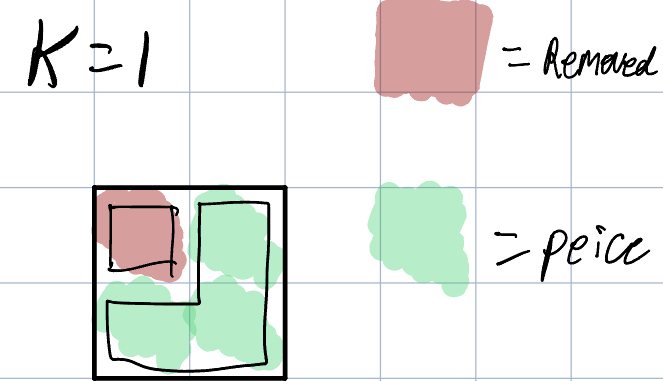
\includegraphics[width=0.5\textwidth]{images/1.1.jpeg}
\end{center}
We can use this as a base case for our
divide and conquer algorithm. We can now move onto if k is greater than 1.
We move onto if k is equal to 2 which equates to $2^2\times2^2=16$ squares. We can first split the board into 4 equal
squares with the top left square removed with each 2x2 square having only 
4 squares execpt for the top left square. We can now see that we can split this 
into smaller subproblems of size 2x2 from the base case. We can simulate a piece
being removed from the corner by putting a L-shaped piece in the middle of the 
board. We can now fill the board with the corresponding piece for each subproblem
as there is only one possible placement. 
\begin{center}
    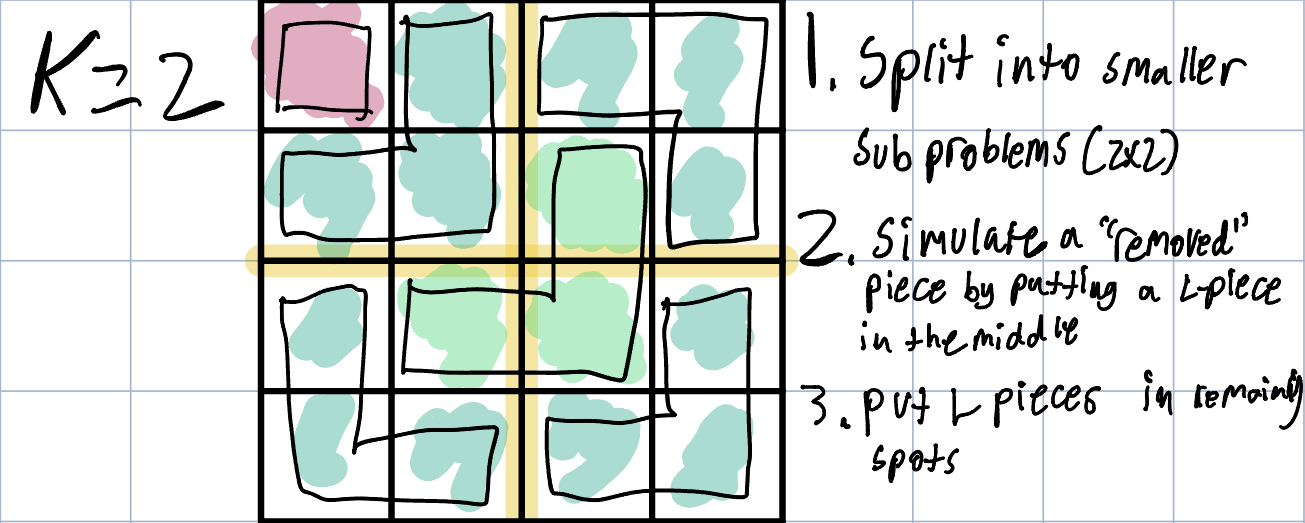
\includegraphics[width=0.5\textwidth]{images/1.2.jpeg}
\end{center}
We can move onto if k is equal to 3 which equates to $2^3\times2^3=64$ squares. We can do the same
process as before by splitting the board into 4 equal squares with the top left square removed leaving
behind 4 4x4 squares (with one of them missing a square).
We can now see that we can split this into even smaller subproblems of size 2x2 which
we can see if the base case. We now can put a L-shaped piece in the middle of each time
we split to simulate a piece being removed from the corner for each 4x4 and 2x2 square.
For the 4x4 squares however the oreintation of the L-shaped piece is different as the middle 
piece that simulates the removed square is in a different position. This however is not a problem
as we can just rotate the piece to fit the square. We can now fill the board with the corresponding
piece for each subproblem which we found from the previous problem.
\begin{center}
    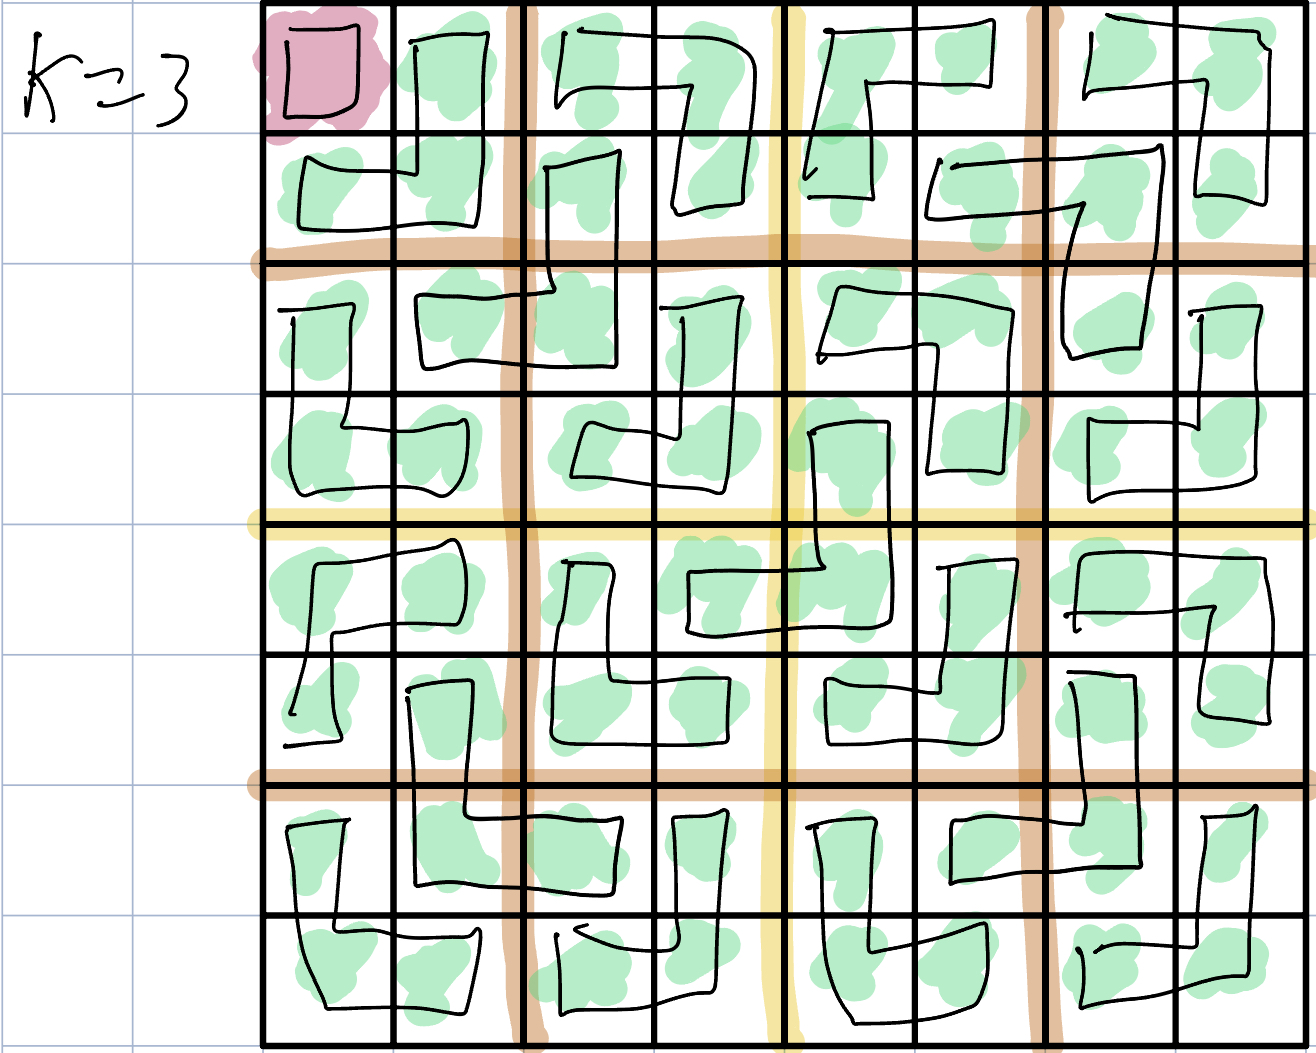
\includegraphics[width=0.5\textwidth]{images/1.3.jpeg}
\end{center}
From all these examples we can derive a pattern that we can use to solve this problem. We split the board into smaller and smaller subproblems until we reach the base.
We can then fill the board with the corresponding piece for each subproblem. From this we can see that this
pattern works for all $k$ as we can just keep splitting the board into smaller and smaller subproblems
until we reach the base case. This means that we can solve this problem by using a divide and conquer
algorithm of splitting the board up. The algorithm is as follows:
\begin{enumerate}
    \item Remove the top left square from the board.
    \item Split the board into 4 equal squares.
    \item For each time you split the board, put a L-shaped piece in the middle of that board.
    \item Repeat steps 2 and 3 until you reach the base case of a 2x2 board for each subproblem.
    \item Fill the board with the corresponding piece for each subproblem.
\end{enumerate}
This algorithm is correct because we are just creating smaller and smaller subproblems that 
simulate the base case of a 2x2 board.

\pagebreak

\section*{Problem 2}

You are given an unsorted list $L$ that has $k \ge 0$ pairs of indices $i < j$ such that $L[i] > L[j]$.
These are called $inverted$ $pairs$. Develop an $O(n log n)$ algorithm that counts the number of
inverted pairs (i.e. compute the value $k$).

\begin{enumerate}
    \item First we can think about how we can count the number of inverted pairs. We can do this by
    using a merge sort algorithm. We can start by splitting the list into two equal parts. We can then
    recursively call the merge sort algorithm on each half of the list. We can now merge the two lists
    together by comparing the first element of each list. We can now see that if the first element of the
    first list is greater than the first element of the second list, then we can see that all the elements
    in the second list are greater than the first element of the first list. This means that we can add
    the number of elements in the second list to the number of inverted pairs. We can now add the smaller
    element to the merged list and remove it from the original list. We can now repeat this process until
    we have merged the two lists together. We can now see that we can count the number of inverted pairs
    by using a merge sort algorithm. This means that we can solve this problem by using a merge sort algorithm.
    \item We can now think about how we can implement a merge sort algorithm. We can start by splitting the list
    into two equal parts. We can then recursively call the merge sort algorithm on each half of the list. We can now
    merge the two lists together by comparing the first element of each list. We can now see that if the first element
    of the first list is greater than the first element of the second list, then we can see that all the elements in the
    second list are greater than the first element of the first list. This means that we can add the number of elements
    in the second list to the number of inverted pairs. We can now add the smaller element to the merged list and remove
    it from the original list. We can now repeat this process until we have merged the two lists together. We can now see
    that we can count the number of inverted pairs by using a merge sort algorithm. This means that we can solve this problem
    by using a merge sort algorithm.
\end{enumerate}

\pagebreak

\section*{Problem 3}
The \textit{best subset problem} is defined as, given a list $(x_1, x_2, \ldots , x_n)$ of integers 
(which can be positive, negative, or zero), find $(i, j)$ such that $x_i + x_{i+1} + \ldots + x_j$ is 
maximum for any $1 \leq i \leq j \leq n.$ For example, if $n = 10$ and the input is $(4, -8, -5, 8, -4, 3, 6, -3, 2, -11)$ 
then the output is $x_4 + x_5 + x_6 + x_7 = 8 - 4 + 3 + 6 = 13.$

\begin{enumerate}
    \item{Develop an $O(n)$ algorithm for the related problem, \textit{best subset middle} or BSM. The input to BSM is a list $(x_1, x_2, \ldots , x_n)$ of integers (which can be positive, negative, or zero) and the output is the maximum value of $x_i + x_{i+1} + \ldots + x_j$ such that $[i, j]$ spans $\frac{n}{2}$, in other words, for all possibilities for $i$ and $j$ such that $1 \leq i \leq \frac{n}{2} \leq j \leq n.$}
    \item{Design a recursive algorithm for the best subset problem with runtime $O(n log n)$ that
    uses the BSM function.}
    \item{Argue that your algorithm is indeed correct and prove the runtime is $O(n log n).$}
    \item{ (Extra credit: 5pts) Design an algorithm for the best subset problem that has $O(n)$
    runtime. Argue why your algorithm is correct and has $O(n)$ runtime.}
\end{enumerate}

\begin{enumerate}
    \item We can solve this problem by using a dynamic programming algorithm. We can start by creating a list 
    of the same size as the input list. We can now set the first element of the list to the first element of the 
    input list. We can now iterate through the input list and set the current element of the list to the maximum of 
    the current element of the list and the current element of the input list plus the previous element of the list. 
    We can now iterate through the list and find the maximum element of the list. This is the maximum sum of the subarray. 
    This means that we can solve this problem by using a dynamic programming algorithm.
    \item We can now think about how we can implement a dynamic programming algorithm. We can start by creating a list 
    
\end{enumerate}

\end{document}
